\chapter{引言}\label{chap:introduction}

% 随着计算机技术的发展,各种指令集架构层出不穷,如X86、ARM、LoongArch\cite{LoongArch2023}、RISCV等。这些指令集之间互不兼容,导致软件需要针对不同架构进行多次开发和编译,无法进行通用迁移,增加了软件开发的成本和复杂度。

David Patterson曾经宣称我们正处于计算机体系结构的一个“黄金时代”\cite{goldenage},这个时期以技术创新和多样性为特征,为研究者和工程师提供了前所未有的机遇来重塑未来的计算机系统。随着计算需求的多样化以及能效、性能比的关注,各种指令集架构(ISA)应运而生,包括众所周知的X86和ARM,以及新兴的LoongArch和RISCV等。这些架构各自针对特定的应用场景、性能需求和能效目标进行了优化设计。

\section{国产CPU指令集碎片化问题}

% https://zhuanlan.zhihu.com/p/599483286 国产CPU的发展现状
中国国产CPU在多个架构上展现出丰富多彩的发展,其中X86、ARM、LoongArch和RISCV等架构代表了不同的技术路线,由各个公司推动。参见表\ref{tab:CPUs},以下是各架构的特点:

% https://www.tablesgenerator.com/latex_tables 生成latex表格
\begin{table}[]
\centering
\caption{国产CPU的发展现状}
\label{tab:CPUs}
    \begin{tabular}{llll}
    \rowcolor[HTML]{FBE5D6} 
    指令集       & 代表公司   & 优势        & 不足         \\
    X86       & 兆芯,海光  & 兼容Windows & 授权问题 \\
    ARM       & 华为,飞腾  & 兼容安卓      & 授权问题       \\
    LoongArch & 龙芯     & 自主可控      & 生态不足       \\
    RISCV     & 开芯院,阿里 & 开源开放      & 生态不足      
    \end{tabular}
    \end{table}


    \begin{itemize}
    \item {X86架构: } 代表公司为兆芯和海光,采用X86架构IP内核授权模式,可基于公版CPU核进行优化或修改,性能起点高,生态壁垒相对低。但是依赖海外企业授权,自主可控风险偏高。
    
    \item{ARM架构:} 代表公司为华为和飞腾,采用Armv8永久授权,具有更高的自主化程度,可自行研发设计CPU内核和芯片,也可扩充指令集。但是存在长期隐患,因为Arm公司将不再向这些国产CPU厂商提供Armv9的永久授权。
    
    \item{LoongArch架构:} 代表公司为龙芯,采用自研的LoongArch指令集,具有相对更高的自主可控程度,已经在党政军工行业得到了广泛应用。但是自研指令集生态不足,需要大量投入才能建立起完善的软件生态。
    
    \item{RISCV架构:} 代表公司为开源芯片研究院和阿里平头哥,采用国际开源的RISCV架构,具有相对精简的指令集架构,并遵循开源宽松的BSD协议,在国内得到了迅速发展,但同样生态不足,需要长时间生态建设。
    \end{itemize}


\begin{figure}[!htbp]
    \centering
    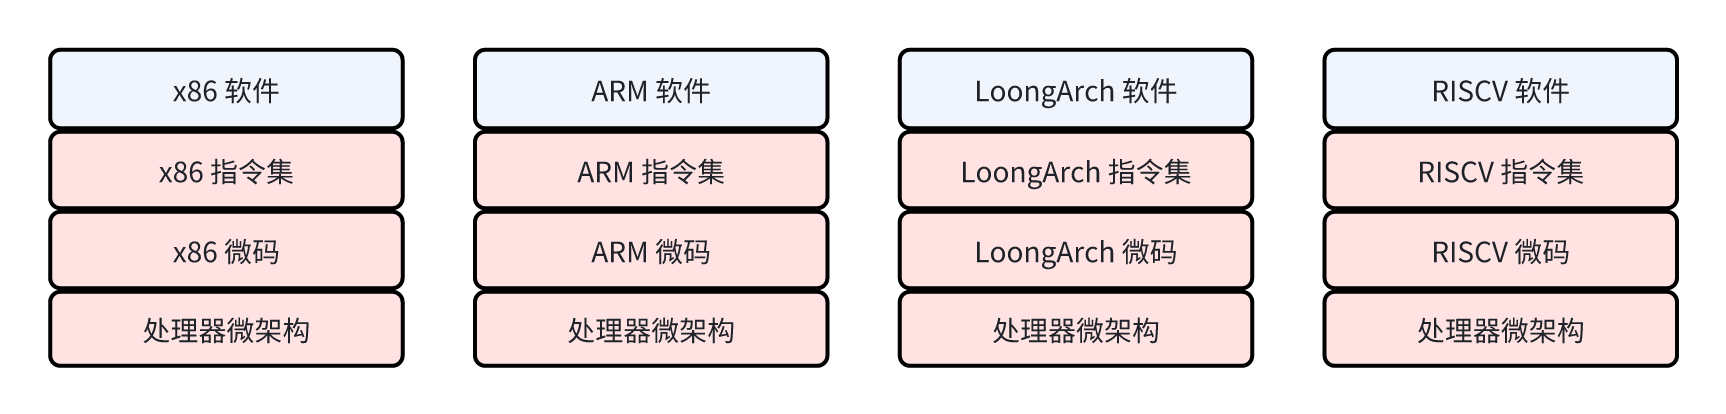
\includegraphics[width=1\linewidth]{./feishuImage/allCPU_arch.png}
    \caption{不同指令集CPU的架构图,图中白色为软件层,红色为硬件层,并忽略了操作系统,这不是本文研究重点。\protect\footnotemark}
    \label{img:allCPU_arch}
  \end{figure}

\footnotetext{ARM, LoongArch, RISCV 等精简指令集架构(RISC)的CPU,内部可以实现微码层,也可以不实现,根据具体CPU微架构实现而不同。}

如图\ref{img:allCPU_arch}所示,同一套软件源代码需要针对不同的指令集进行编译才能在不同架构的CPU上运行\footnotemark。

\footnotetext{这里主要关注C/C++等底层语言,对于Java等支持跨平台运行的语言,也需要Java虚拟机对不同指令集平台进行编译适配。}

    而中国国产CPU的多样性导致了指令集的碎片化,增加了应用程序在不同架构间迁移和适配的复杂性。存在的问题包括:
    \begin{itemize}
    \item \textbf{适配和迁移负担:} 不同架构间的适配和迁移需要大量人力和物力资源。
    
    \item \textbf{历史兼容包袱:} 不同指令集的历史兼容包袱使得跨架构的兼容性复杂。
    
    \item \textbf{编译与源代码的限制:} 古老软件无源代码,只能通过翻译运行以适应新的指令集。
    
    \item \textbf{操作系统支持的挑战:} 操作系统厂商需要投入更多资源以支持不同架构。
    \end{itemize}

\section{二进制翻译器概述}
目前,二进制翻译技术是解决指令集兼容性问题的主要方法。

\begin{figure}[!htbp]
  \centering
  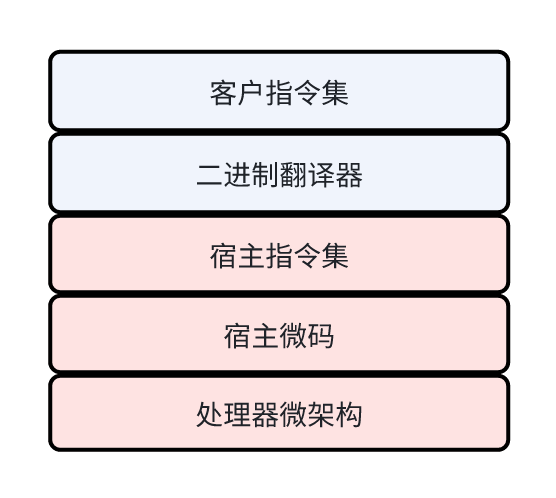
\includegraphics[width=0.3\linewidth]{./feishuImage/BT_arch.png}
  \caption{二进制翻译器架构图,能在宿主指令集机器上运行客户程序。}
  \label{img:BT_arch}
\end{figure}

如图\ref{img:BT_arch} 二进制翻译技术能够将一个指令集(称为客户指令集)上的二进制程序翻译到另一种指令集(称为宿主指令集)上执行,
而二进制翻译器有多种不同的分类方式,如静态与动态、用户态与系统态、解释型与翻译型、软件实现与软硬件实现等,这些分类方式可以根据不同的需求和应用场景进行组合,并且基本是\textbf{正交}的。

下面是对这些分类的简要说明:

\subsection{静态与动态}
静态二进制翻译:在程序执行前,将整个源程序从一种机器指令集转换到另一种。这种转换通常产生新的可直接执行文件,无需在运行时进行额外的转换。
静态翻译的优点在于它可以在转换过程中进行深入的代码分析和优化,但它不适用于动态生成代码的情况,也不能处理代码数据混淆等复杂的情况。

动态二进制翻译:在程序运行时,按需将代码从源指令集转换为目标指令集。这种方法适用于处理动态生成的代码,如即时编译(JIT)产生的代码。
动态翻译可以实现更高的灵活性和与特定硬件环境的即时优化,但会引入额外的运行时开销。

\begin{figure}[!htbp]
  \centering
  \includegraphics[width=1\linewidth]{./image/sbt_dbt.pdf}
  \caption{左图为静态二进制翻译器,在运行前提前翻译成预翻译文件,运行时直接执行。右图为动态二进制翻译器,在运行时翻译基本块并存入代码缓存,翻译过的基本块就直接执行。}
  \label{img:sbt_dbt}
\end{figure}

两者的概念图可以看\ref{img:sbt_dbt}。

\subsection{用户态与系统态}
用户态二进制翻译:仅转换用户空间程序的指令,不涉及操作系统核心态的代码。这种翻译对于实现应用程序的跨架构兼容性特别有用,相对于系统态翻译,性能更高。

系统态二进制翻译:模拟整个系统,包括CPU、内存、设备等,能够转换操作系统内核代码和驱动程序,以实现整个操作系统的兼容。这要求翻译器能够处理更为复杂的系统级别的操作,如中断处理和系统调用。

\begin{figure}[!htbp]
  \centering
  \includegraphics[width=0.8\linewidth]{./image/user_sys.pdf}
  \caption{左图为用户态二进制翻译器,只需运行客户程序。右图为系统态二进制翻译器,其上需要运行整个客户操作系统。}
  \label{img:user_sys}
\end{figure}

两者的概念图可以看\ref{img:user_sys}。

\subsection{解释型与翻译型}
解释型二进制翻译:通过逐条解释源指令并立即执行对应的目标指令来运行程序。这种方式可以实现较高的兼容性,因为它可以逐步处理源程序的每个指令,但其性能通常低于直接执行。一般用于调试、模拟和验证等场景。

翻译型二进制翻译:将源程序的指令以基本块为单位翻译成目标机器的指令,然后执行翻译后的代码。这种方法在翻译阶段可能会花费更多时间,但运行翻译后的代码的速度更快。

\begin{figure}[!htbp]
  \centering
  \includegraphics[width=1\linewidth]{./image/inter_bt.pdf}
  \caption{左图为解释型二进制翻译器,以单条指令为单位,解释指令语义执行。右图为翻译型二进制翻译器,以基本块为单位,翻译整个基本块并进行优化后执行。}
  \label{img:inter_bt}
\end{figure}

两者的概念图可以看\ref{img:inter_bt}。

\subsection{软件实现与软硬件实现}
软件实现:通过软件工具和技术完全在软件层面上实现二进制翻译。这种实现方式的优点在于其灵活性和可移植性,但可能会因为缺乏硬件支持而影响翻译性能。

软硬件实现:结合使用专门的硬件支持和配套的软件技术来提高二进制翻译的效率。例如,通过在处理器中实现特定的硬件间接跳转表来加速间接跳转的翻译执行\cite{Godson3}。这种方法可以显著提高性能,但增加了硬件设计的复杂性和成本。

表\ref{tab:BTs}对这些分类进行了总结,
各种二进制翻译技术的选择取决于特定应用的需求、目标架构的特性以及性能和兼容性之间的权衡。

\begin{table}[]
  \caption{二进制翻译技术的分类及优劣势比较}
  \label{tab:BTs}
  \begin{adjustbox}{width=\textwidth}
  \begin{tabular}{llll}
  \rowcolor[HTML]{FFCE93} 
      & 说明                  & 优势           & 不足                  \\
  静态  & 提前翻译                & 深入的代码分析和优化   & 无法处理动态生成代码,首次翻译时间长  \\
  动态  & 运行时翻译和优化            & 能处理动态生成代码    & 额外的运行时开销,无法做重型优化    \\
  \hline
  用户态 & 只翻译用户态指令            & 实现简单,性能较高    & 不能翻译操作系统,支持应用有限     \\
  系统态 &  模拟整个系统 & 能直接跨架构运行操作系统 & 性能较低                \\
  \hline
  解释型 & 逐条指令解释执行            & 方便调试模拟等      & 性能很低,一条指令会解释为10余条指令 \\
  翻译型 & 一般以基本块为单位翻译执行       & 性能较高         & 设计更加复杂              \\
  \hline
  软件  & 纯软件实现               & 灵活性和可移植性     & 性能不高                \\
  软硬件 & 特定硬件支持    & 特定硬件加速提升性能   & 增加硬件设计复杂性          
  \end{tabular}
  \end{adjustbox}
  \end{table}

目前主流的二进制翻译器一般采用\textbf{动态、用户态、翻译型和软件实现}的方式,如QEMU\cite{bellardQEMUFastPortable2005}、Rosetta2\cite{RosettaTranslationEnvironment, RunningIntelBinaries}、ExaGear\cite{KunPengExaGear}、LATX\cite{LoongArchEnv2022, LoongArch2023}等,这是由于动态翻译可以在运行时进行优化并能支持JIT程序的翻译运行,用户态翻译、翻译型翻译可以实现更高的性能,软件实现可以实现更好的可移植性。


% \section{二进制翻译器性能问题}
但是由于现有的开源二进制翻译器性能
\footnote{
    目前工业界和学术界对二进制翻译的性能有着默认统一的定义:同一份测试程序的源码用相同编译参数,编译到客户指令集和宿主指令集,得到两份二进制文件$B_g$和$B_h$。
    在硬件平台用二进制翻译运行客户程序$B_g$的时间记为$T_{bt}$,在同一硬件平台直接运行宿主程序$B_h$的时间记为$T_h$。
    二进制翻译的性能则为翻译运行时间除以原生运行时间$\frac{T_{bt}}{T_h}$。
}
相对较低,例如QEMU\cite{bellardQEMUFastPortable2005}虽然支持多架构应用,但在翻译运行SPEC CPU 2017\cite{SPECCPU2017}程序时候,仅有约10\%的性能。商业二进制翻译器也存在性能损失,
如苹果的Rosetta2\cite{RosettaTranslationEnvironment, RunningIntelBinaries}、
华为的ExaGear\cite{KunPengExaGear}、
和龙芯的LATX\cite{LoongArchEnv2022, LoongArch2023},
性能仅达到原生运行的70\%左右,并且仅能保证单一指令集翻译到单一指令集,并不通用,多架构支持较为困难,这直接影响了软件生态迁移的流畅度和成功性,
后文\ref{chap:related_work}会详细分析现有二进制翻译器的开销来源。

% \section{多架构软硬协同二进制翻译的需求}
\section{本文的主要工作及贡献}

为了解决\textbf{指令集碎片化}和\textbf{二进制翻译器性能}问题,迫切需要多架构软硬协同的二进制翻译技术。这项技术的关键目标是在同一套硬件下实现多指令集的共存,为软件提供更好的跨平台兼容性和性能表现。

如图\ref{img:my_arch}所示,本团队提出了一种多架构软硬协同的二进制翻译技术——\textbf{微译器},按照上述分类属于\textbf{动静结合、用户态、翻译型、软硬结合},
通过在硬件层面支持一套融合微码,为软件层面的二进制翻译器提供更好的性能和兼容性。


\begin{figure}[!htbp]
    \centering
    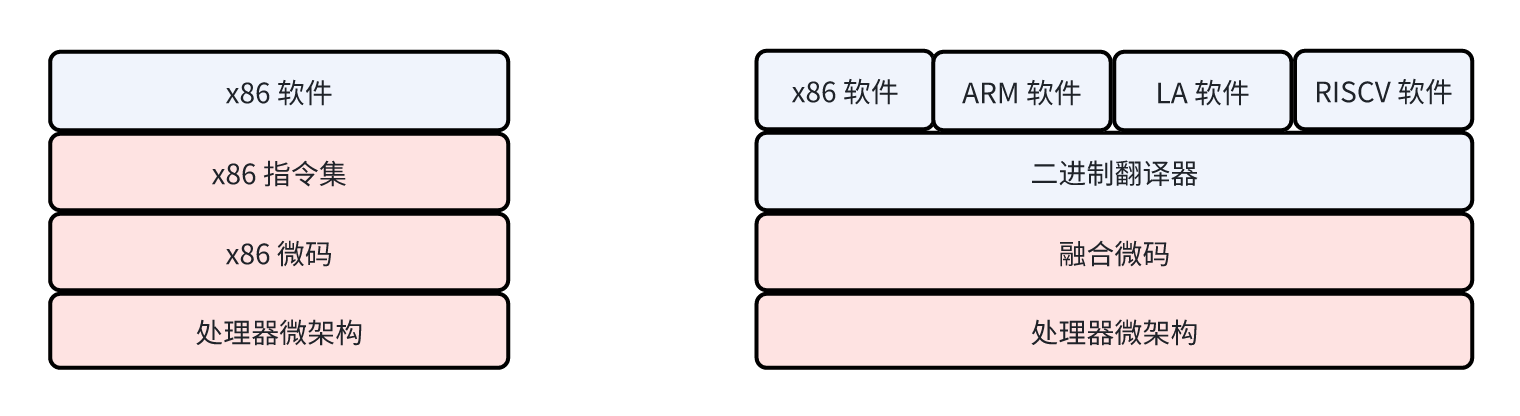
\includegraphics[width=1\linewidth]{./feishuImage/my_arch.png}
    \caption{多架构软硬协同的二进制翻译架构图,硬件仅对外暴露微码,软件层面的二进制翻译器可以实现多架构的支持,性能接近原生运行性能。}
    \label{img:my_arch}
  \end{figure}

这项技术的优势在于:

1. \textbf{打破指令集边界,消除应用迁移成本:} 应用程序无需适配和迁移至特定指令集,可直接在同一套硬件上运行,降低了软件开发和维护的复杂性。

2. \textbf{硬件对外暴露微码,规避X86等授权问题:} 通过在硬件层面暴露微码,技术在一定程度上规避了X86等架构的授权问题,提高了国产CPU的自主性。

3. \textbf{软件维护历史兼容,微码迭代优化:} 作为软件层面的核心组件,二进制翻译器维护历史兼容性并实现微码迭代优化,确保不同架构的硬件在不同历史时期的应用中保持高效运行。

本文的主要工作及贡献如下:

1. 合作提出了一种多架构软硬协同的二进制翻译技术——微译器,实现了多架构的支持,为软件提供了更好的跨平台兼容性和性能表现。

2. 在微译器已有的支持X86翻译执行的框架下,添加RISCV架构的支持,用于验证微译器对多架构支持的可行性和性能表现。

3. 优化微译器的性能,包括对微码缓存的优化,融合微码的压缩指令集设计,旨在缓解微码缓存导致的代码膨胀问题。


\section{论文的组织结构}
% 本文在第二章介绍二进制翻译相关工作,包括软硬协同二进制翻译器和纯软件二进制翻译器。第三章介绍微译器的架构设计和实现,第四章介绍在微译器中添加RISCV架构的实现,第五章介绍微译器优化方案,第六章介绍微译器的性能测试和分析,第七章总结全文并展望未来工作。

本文的组织结构如下:

在第二章介绍二进制翻译的相关工作,包括软硬协同二进制翻译器和纯软件二进制翻译器,并对二进制翻译器的性能开销进行分析,发现间接跳转的性能开销以及指令集语义差异是二进制翻译器性能的主要瓶颈。
进而为了解决间接跳转的问题,引出了复杂指令集X86处理器的微码缓存的概念,为微译器的设计提供了设计思路。

第三章介绍团队项目——微译器的架构设计和实现,包括微译器的整体架构和实现,微码缓存的设计和实现,融合微码的设计思想。

第四章介绍本文在微译器中添加RISCV架构的实现,包括RISCV和X86的指令集语义差异,系统调用相关的ABI差异,以及微译器的多架构支持的实现。

第五章介绍微译器的优化方案,这里特指引入微译器后产生的额外性能开销的优化方案,包括微码缓存的优化,融合微码的压缩指令集设计,旨在缓解微码缓存导致的代码膨胀问题。

第六章介绍微译器的性能测试和分析,包括微译器的实验环境,调试环境,性能测试结果的分析和讨论。

第七章总结全文并展望未来工作。

aaaaaa

aaaaaa

aaaaaa

aaaaaa

aaaaaa

aaaaaa
aaaaaa

aaaaaa

aaaaaa

aaaaaa

aaaaaa

aaaaaa